\todo[inline]{TODO: I plan to add description and section headings over break}
\todo[inline]{TODO: add discussion of powerstroke vs winch models. Discuss simple modifications to simulation parameters to try and fit for this alternate mechanochemical model}

\todo[inline]{TODO: combine 5.1 with 5.2 to explain leading vs lagging}
\todo[inline]{TODO: consider removing leading lagging axis labels in 5.1 if redundant with figure caption} 
\todo[inline]{NOTE: it looks like there may be an issue with the middle most cartoon in 5.3. The tail does not appear to be the correct size}
\todo[inline]{TODO decrease overall width of tail in cartoon dynein. Increase thickness of stalk} 
\todo[inline]{TODO: Check to make sure time axis in final panel of fig 5.4 is actually a log scale} 

\section{Best-fit parameters}
\section{Stepping}
\begin{figure}
	\centering
	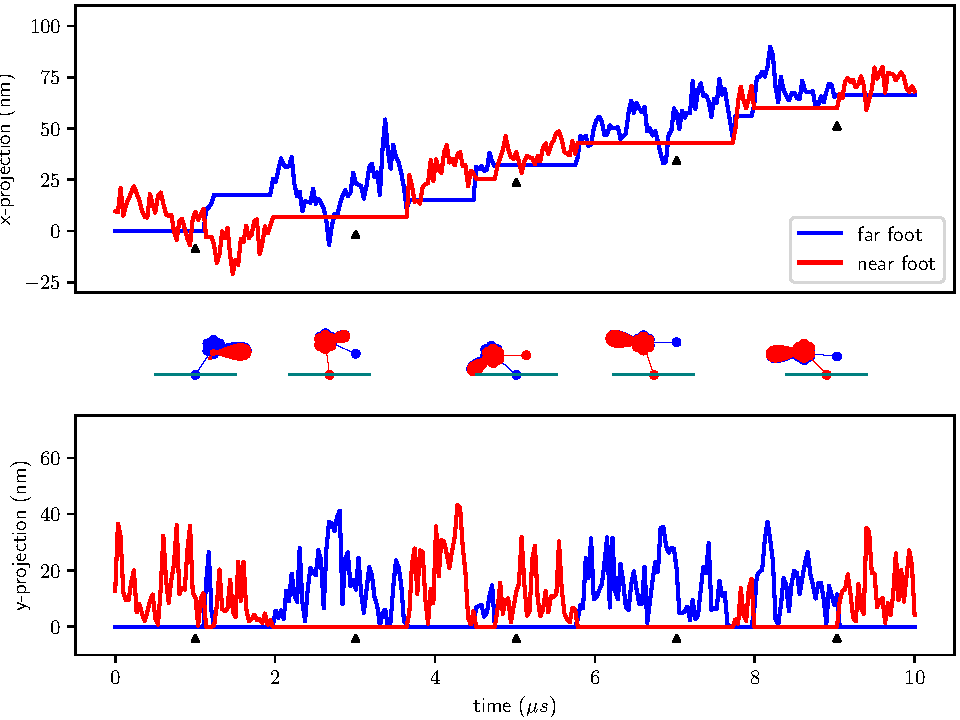
\includegraphics[width=1\columnwidth]{paper_trajectory_plot}
	\caption{\textbf{Trajectory Plot} Vertical and horizontal projections of each of binding domains. Directed motion is clearly seen in the positive slope of the x-projection graph. Dynein's conformation is illustrated for a selection of times.}
	\label{fig:trajectory}
\end{figure}
	
	
\begin{figure}
	\centering
	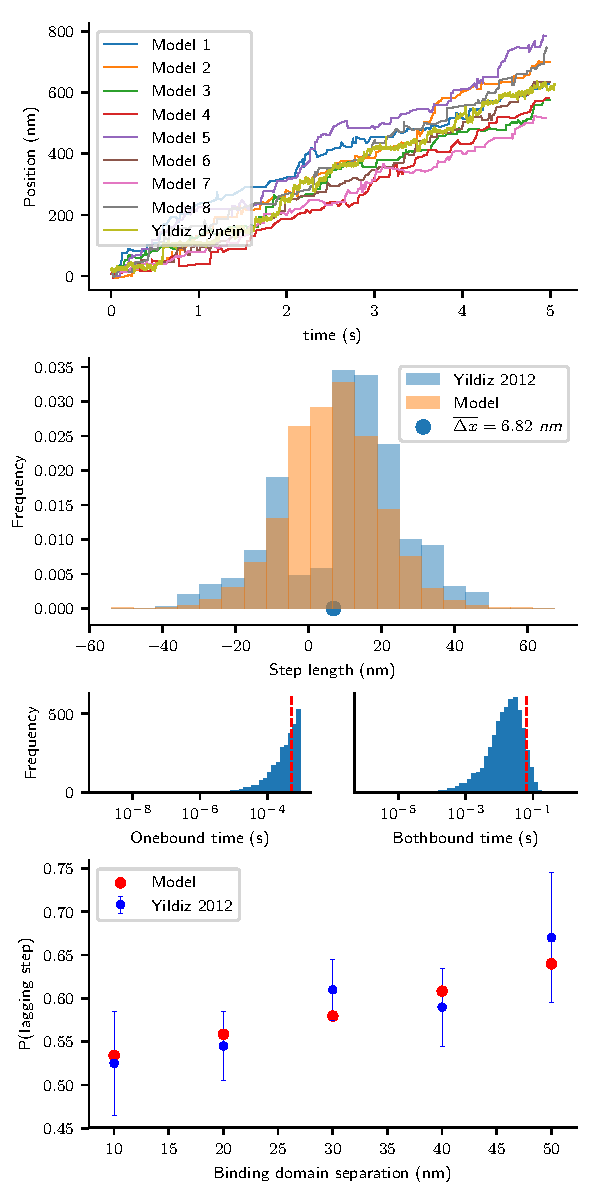
\includegraphics[width=0.85\columnwidth]{paper_model_behavior}
	\caption{\textbf{Stepping statistics} trajectories run with different random number seeds all show forward directed motion. Step lengths have a similar distribution to experiment although steps of zero length are not measured experimentally. }
	\label{Fig:statistics}
\end{figure}


\section{One bound and both bound correlations}
\begin{figure}[!hbt]
	\centering
	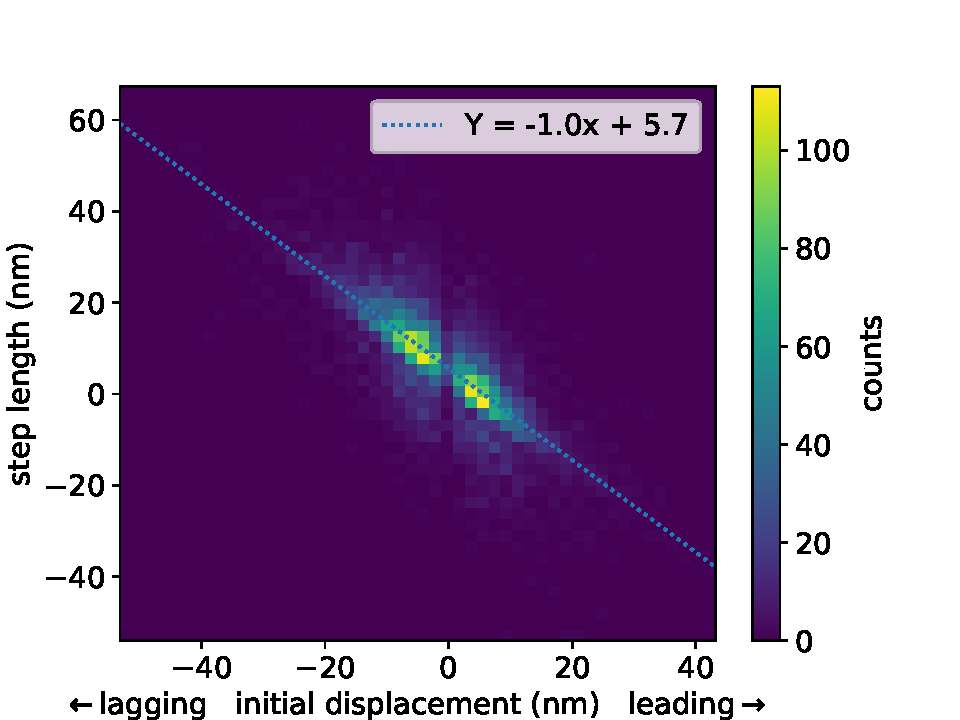
\includegraphics[width=0.75\columnwidth]{paper_displacement_vs_step_length}
	\caption{\textbf{Two dimensional histogram} comparing the total signed step length to
			the signed initial displacement between the binding domains. A positive value
			indicates that the front foot made the step (leading). A negative value
			indicates the rear foot (lagging) made the step. Simulations show a strong,
			negative correlation. A similar fit from an experimental paper is plotted for comparison.}
	\label{fig:displacement_vs_step_length}
\end{figure}
	
	
\begin{figure}[!hbt]
	\centering
	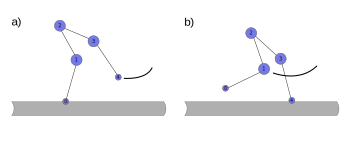
\includegraphics[angle=-90, width=1\columnwidth]{leading_vs_lagging}
	\caption{Diagram illustrating a leading foot step (a) and a lagging foot step (b).}
\end{figure}



\section{Possible Monte Carlo}
\begin{figure}[!hbt]
	\centering
	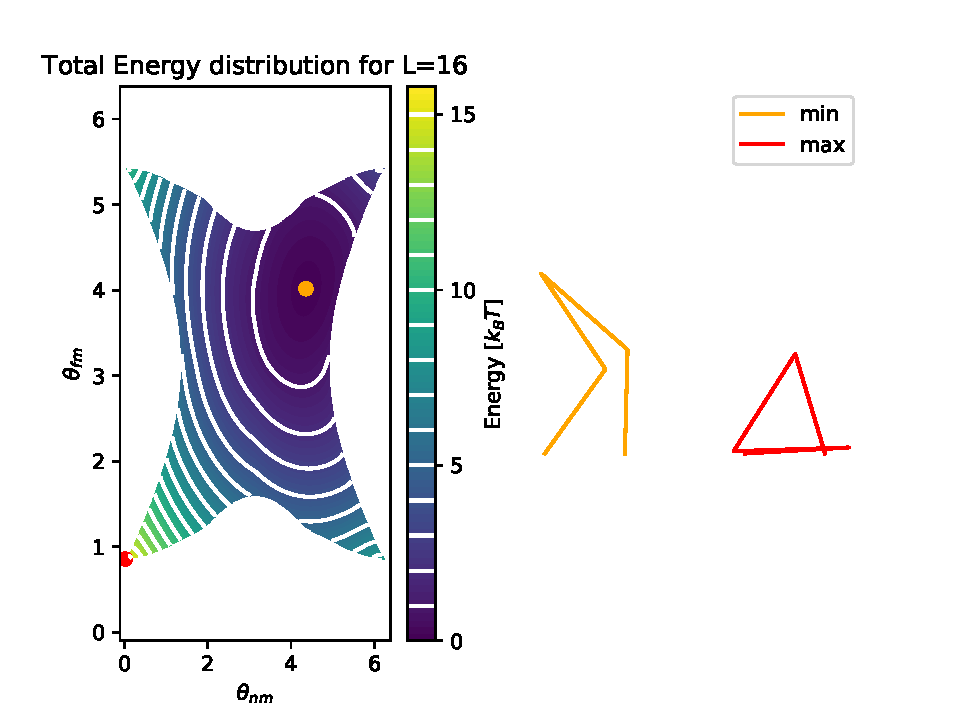
\includegraphics[width=1\columnwidth]{energy_landscape}
	\caption{\textbf{Energy Landscape} graph showing the total energy of the dynein for a given binding domain displacement $L$. The yellow and red dots correspond to the minimum and maximum energy configurations for which a cartoon is shown on the right.}
	\label{fig:energy_landscape}
\end{figure}


			

\vspace{10em}
